% !TEX program = xelatex
% akizumi-tikz in slides: theme options tikz=full and plots
\documentclass[aspectratio=169,11pt]{beamer}
\usetheme[tikz=full, plots]{Akizumi}
\begin{document}
\begin{frame}{Diagrams}
  \begin{tikzpicture}[akizumi/automaton]
    \node[state, initial] (a) {$a$};
    \node[state, accepting, right=of a] (b) {$b$};
    \path[->] (a) edge["$0$"] (b);
  \end{tikzpicture}
  \quad
  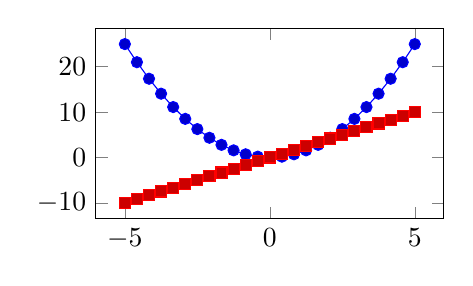
\begin{tikzpicture}
    \begin{axis}[width=6cm, height=4cm]
      \addplot {x^2}; \addplot {2*x};
    \end{axis}
  \end{tikzpicture}
\end{frame}
\end{document}
